%%%%%%%%%%%%%%%%%%%%%%%%%%%%%%%%%%%%%%%%%%%%%%%%%%%%%%%%%%%%%%%%%%%%%%%%%%%%%%%
% Chapter 3: Procedimiento experimental 
%%%%%%%%%%%%%%%%%%%%%%%%%%%%%%%%%%%%%%%%%%%%%%%%%%%%%%%%%%%%%%%%%%%%%%%%%%%%%%%


%++++++++++++++++++++++++++++++++++++++++++++++++++++++++++++++++++++++++++++++
\section{Descripci�n de los experimentos}
\label{3:sec:1}

En los experimentos, el tiempo de c�lculo depende del ordenador, los intervalos, y el error que utilicemos, por ello explicaremos eso junto con el c�digo.

\*Ver Ap�ndice A.1. (Codigo \textsf{Python})


%++++++++++++++++++++++++++++++++++++++++++++++++++++++++++++++++++++++++++++++
\section{Descripci�n del material}
\label{3:sec:2}

('default', 'Feb 27 2014 20:00:17')

Linux-3.2.0-61-generic-i686-with-Ubuntu-12.04-precise

('Linux', 'FISICA-PC', '3.2.0-61-generic', '#93-Ubuntu SMP Fri May 2 21:33:33 UTC 2014', 'i686', 'i686')

2.7.3

Genuine Intel(R) CPU            2160  @ 1.80GHz

GenuineIntel

1200.000 Hz

1024 KB

\*Ver Ap�ndice A.2.(Codigo \textsf{Python} para el Hardware)

%++++++++++++++++++++++++++++++++++++++++++++++++++++++++++++++++++++++++++++++
\section{Resultados obtenidos}
\label{3:sec:3}

Al realizar la bisecci�n de la funci�n, obtenemos una serie de datos.
Un claro ejemplo es el c�lculo del tiempo de error. 
Otros de estos datos son las ra�ces calculadas, y otros son simples puntos calculados al sustituir un valor de x en f(x). Con estos puntos podemos realizar las siguientes tabla y gr�fica.


%------------------------------------------------------------------------------
\begin{figure}[!th]
\begin{center}
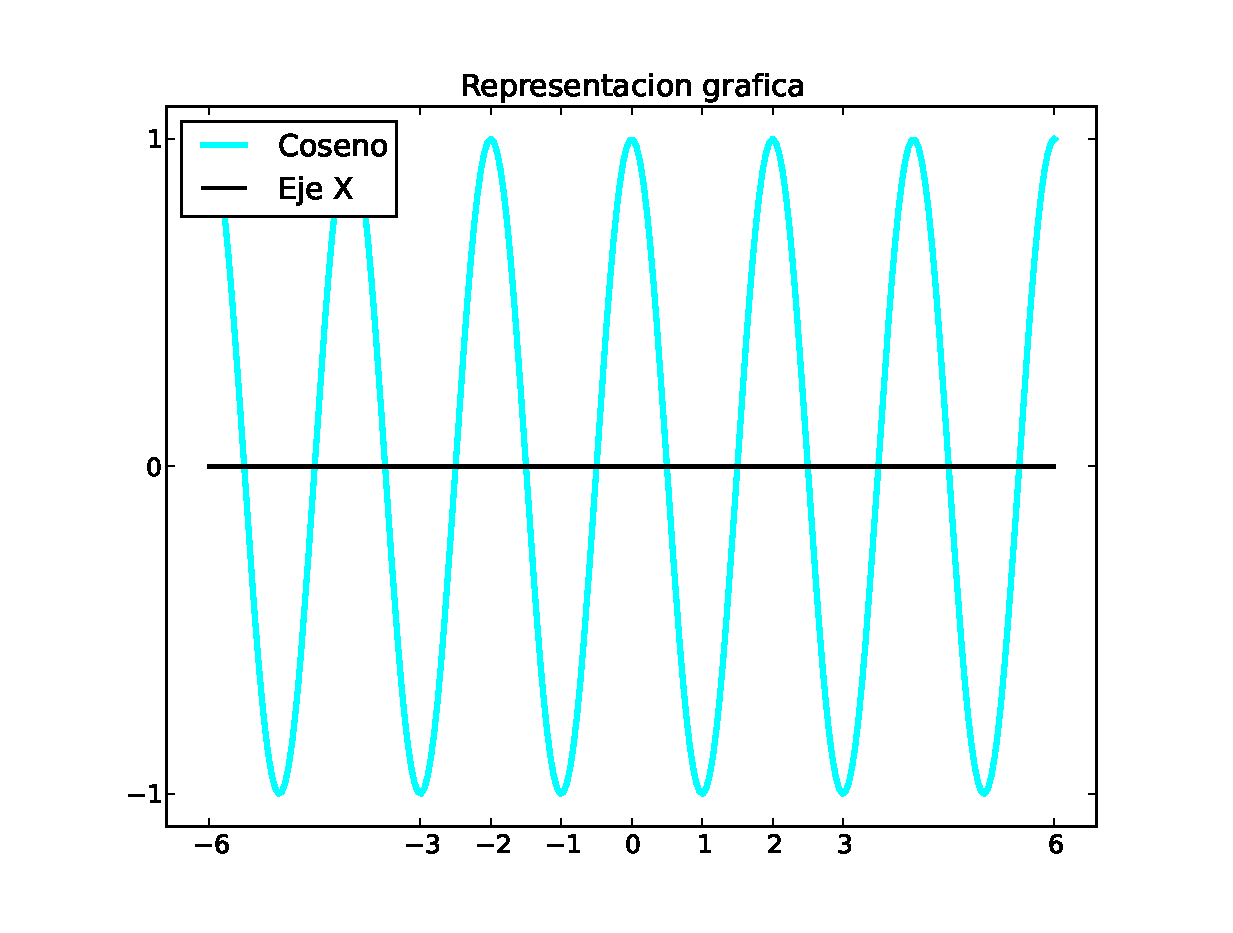
\includegraphics[width=0.5\textwidth]{cos.eps}
\caption{Ejemplo de figura}
\label{fig:1}
\end{center}
\end{figure}
%------------------------------------------------------------------------------
\begin{figure}[!ht]
\begin{center}
\includegraphics[width=0.75\textwidth]{images/imagen1.eps}
\caption{Ejemplo de figura con gr�fico}
\label{fig}
\end {center}
\end {figure}

%------------------------------------------------------------------------------
%--------------------------------------------------------------------------
\begin{table}[!ht]
\begin{center}
\begin{tabular}{|l|c|c|} \hline 

 X    &  Y \\ \hline
- 2   &  1 \\ \hline
 -1.5 &  0 \\ \hline
 -1   & -1 \\ \hline
 -0.5 &  0 \\ \hline
  0   &  1 \\ \hline
  0.5 &  0 \\ \hline
  1   & -1 \\ \hline
  1.5 &  0 \\ \hline
  2   &  1 \\ \hline
  
\end{tabular}
\end{center}
\caption{Datos de f(x)}
\label{tab:1}
\end{table}

\begin{table}[!ht]
\begin{center}
\begin{tabular}{|l|c|c|}
\hline
 X    &  Y \\ \hline
- 2.5 &  0 \\ \hline
 -1.5 &  0 \\ \hline
 -0.5 &  0 \\ \hline
  0.5 &  0 \\ \hline
  1.5 &  0 \\ \hline
  2.5 &  0 \\ \hline
\end{tabular}
\end{center}
\caption{Algunas raices de f(x)}
\label{tab}
\end{table}


%------------------------------------------------------------------------------

%++++++++++++++++++++++++++++++++++++++++++++++++++++++++++++++++++++++++++++++
\section{An�lisis de los resultados}
\label{3:sec:4}

Como sabemos, lo que conseguimos con la bisecci�n es calcular las ra�ces de la funci�n tratada.
Dependiendo del intervalo dado y el margen de error,  este valor se aproximar� de mejor o peor modo, pero despu�s de utilizar este programa realizado en \textsf{Python} podemos dar una tabla de ra�ces de nuestra funci�n, que al ser periodica tiene infinitas.

